%======================================================================
%----------------------------------------------------------------------
%               XX                              X
%                                               X
%               XX    XXX   XXX   XXX      XXX  X  XXXX
%                X   X   X X   X X   X    X   X X X
%                X   XXXXX XXXXX XXXXX    X     X  XXX
%                X   X     X     X     XX X   X X     X
%               XXX   XXX   XXX   XXX  XX  XXX  X XXXX
%----------------------------------------------------------------------
%  	         A SKELETON FILE FOR IEEE PAPER GENERATION
%----------------------------------------------------------------------
%======================================================================

% first, uncomment the desired options:
\documentclass[%
				10pt,
        %draft,
        %submission,
        %compressed,
        final,
        %
        %technote,
        %internal,
        %submitted,
        %inpress,
        %reprint,
        %
        %titlepage,
        notitlepage,
        %anonymous,
        narroweqnarray,
        inline,
        twoside,
        ]{ieee}
%
% some standard modes are:
%
% \documentclass[draft,narroweqnarray,inline]{ieee}
% \documentclass[submission,anonymous,narroweqnarray,inline]{ieee}
% \documentclass[final,narroweqnarray,inline]{ieee}

% Use the `endfloat' package to move figures and tables to the end
% of the paper. Useful for `submission' mode.
%\usepackage {endfloat}

% Use the `times' package to use Helvetica and Times-Roman fonts
% instead of the standard Computer Modern fonts. Useful for the 
% IEEE Computer Society transactions.
% (Note: If you have the commercial package `mathtime,' it is much
% better, but the `times' package works too).
%\usepackage {times}

% In order to use the figure-defining commands in ieeefig.sty...
\usepackage{ieeefig}

% Added Margins
\usepackage[left=1.5in, right=1.5in, top=1.0in, bottom=1.0in]{geometry}
\usepackage{layout}

\begin{document}

%----------------------------------------------------------------------
% Title Information, Abstract and Keywords
%----------------------------------------------------------------------
\title[Reputation Management with Distributed Brokers]{%
       Reputation Management  in Peer to Peer Cloud Storage Utilizing Virtual Currency Exchange and Distributed Brokers}

% format author this way for journal articles.
%\author[SHORT NAMES]{%
%      Bryan Olivas\member{Student Member}
%      \authorinfo{%
%      A. Author is with the Department of Electrical Engineering,
%      Some University, Somewhere CA, 90210, USA,
%      Phone: \mbox{(xxx) xxx-xxxx}, email: \mbox{xxx@xxxx.xxx.xxx}}
%    \and
%      Jiawei Li\member{Student Member}
%      \authorinfo{%
%      B. Author is with the Department of Electrical Engineering...}
%    \and
%      and Vance Thornton\member{Student Member}
%      \authorinfo{...}
%  }

% format author this way for conference proceedings
\author{%
      Bryan Olivas
    \and
      Jiawei Li
    \and
      and Vance Thornton
}

% specifiy the journal name
%\journal{IEEE Transactions on Something, 1997}

% Or, when the paper is a preprint, try this...
%\journal{IEEE Transactions on Something, 1997, TN\#9999.}

% Or, specify the conference place and date.
%\confplacedate{Ottawa, Canada, May 19--21, 1997}

% make the title
\maketitle               

% do the abstract
\begin{abstract}
Virtual currency is a powerful tool for encouraging cooperation in a peer to peer cloud storage service.  In this paper we present a design for a P2P storage system which utilizes a virtual currency for reputation management and compare it to existing currency based P2P reputation management systems.  Our system offers several advantages over existing systems.  One of the most significant of these is that we utilize a distributed broker to help ensure that the nodes participating in a data transfer transaction fulfill their obligations.  Several types of possible attacks on the system are analyzed and a simulation is used to measure the expected effectiveness of the system.
\end{abstract}

% do the keywords
\begin{keywords}
reputation management, peer-to-peer, virtual currency, distributed broker
\end{keywords}

%----------------------------------------------------------------------
% SECTION I: Introduction
%----------------------------------------------------------------------
\section{Introduction}

\PARstart Data storage and transfer play a significant role in many cloud computing applications.  Cloud storage services such as Amazon S3, while very popular, do not necessarily represent the most desirable model for all cloud storage applications.  One issue with such services is limited transparency.  In many cases the source code for the software that is used to provide the service is not made available to the public and so is not available for wide public verification.  Users of the service must trust that the software is sufficiently bug free and secure.  Another drawback to such services is relatively centralized control over physical infrastructure.  All other things being equal it would be preferable if more than one organization was responsible for providing and protecting this infrastructure.  Users can mitigate this issue by storing their data in multiple storage clouds, but this can entail additional cost and complexity.  The cost associated with data storage and transfer is a significant barrier in many applications.  Using a peer to peer network for cloud data storage can potentially eliminate these issues.  If the software is open source then there is a high degree of transparency and a wide community can participate in the verification of the software.  Peer to peer systems are also highly decentralized (Fig. 1).  No single company or individual controls the infrastructure.  Finally if peers are motivated to cooperate the data storage and transfer costs are shared by the peers in a way that can be proportional to the benefit they receive.  Peer to peer cloud storage can make possible applications that would have otherwise been financially infeasible. 

One of the central problems in peer-to-peer systems is ensuring that peers contribute to the system.  For our system design we focus on a virtual currency based approach to this problem.  Virtual currency provides a natural means of tracking the transfer of value between peers.  When a peer provides resources to another peer it receives currency that it can use to acquire resources from other peers.  As with currency in the real world every transaction carries the risk that either the buyer or seller will not provide what was promised.  A broker is an entity that can used to mitigate this risk by acting as a trusted third party that performs the actual exchange on behalf of the buyer and seller.  In this paper we present a design for a peer-to-peer storage system that has brokered virtual currency transactions.  The broker in our system design is distributed to the peers in the network rather than centralized.  This lack of centralization makes the system more robust because a potential single point of failure is eliminated.  Involving more nodes in the broker role also makes the broker more trustworthy.  It is more likely that a few nodes could be malicious or compromised than that the majority of a large number of nodes would be so.  The use of a broker is particularly well suited to peer-to-peer storage because the broker can utilize hashes and encryption keys to verify and perform the transfer.

\begin{figure}
  \begin{center}
    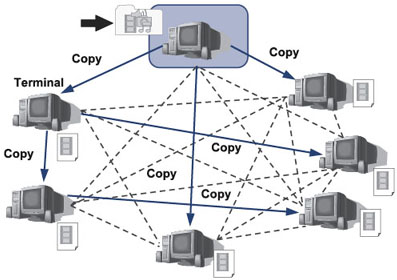
\includegraphics[height=45mm,width=55mm]{graphics/P2PNetwork.jpg}
  \caption{A decentralized storage peer to peer network.}
  \end{center}
\end{figure}

%----------------------------------------------------------------------
% SECTION II: Related Work
%----------------------------------------------------------------------
\section{Related Work}

\subsection{Existing Currency-Based P2P Reputation Management Systems}
P2P has experimented with various schemes and incentives in order to persuade nodes into resource cooperation.  Those in the P2P community have identified these as "Incentive-Based Protocols".  These protocols aim to give incentives or payoffs to nodes in order to make them cooperate ~\cite{gupta}.  The idea is to reward a node with an agreed upon type of credit or virtual currency for their contribution of shared resources.  Some implementations have implored the notion that the reputation of a node is a decaying function of time ~\cite{gupta}.  This would require that a node continuously share resources or provide services.  This can lead to the formation of trust groups.  These can be viewed as trusted communities of nodes.  Each member of a trust group shares the same reputation.  This also means that the individual node store information about every other node in the system.  This, however, may not scale well.  The question remains; how to maintain a fair voluntary resource sharing amongst individual peers.  Currency-based P2P reputation management attempts to solve this.  There are varying factors.  The system must have mechanisms to deal with these factors.  The system needs to manage the challenges of malicious, selfish (rational), altruistic, and free-rider (freeloader) nodes.  The system also must manage the transfer of currency.  We will discuss some of the various systems.  

Dandelion ~\cite{sirivianos} implements P2P static content distribution that relies on security, specifically symmetric cryptography, to provide robust incentives to individual peers.  There exists a server, trusted third party, that maintains a virtual economy.  Each peer has a credit balance.  The server attracts selfish clients by rewarding them with virtual credit for contributing resources.  Inversely the server charges clients for consuming resources from selfish clients.  Transactions are separated into chunks.  If the client has enough virtual credit then that client may acquire a resource chunk.  The system uses encryption and decryption of the data to serve as proof that the exchange has been completed appropriately.  

KARMA ~\cite{vishnumurthy} proposes a framework to avoid freeloaders.  This is accomplished by keeping track of resource contribution and consumption of a given node.  This observation is represented by a scalar value that they call karma.  Nodes are given incentives for contributing resources to a global pool.  The system accounts for the amount of resources that a node has contributed and the amount the node has consumed.  The peer's standing is stored within a global system.  Groups of nodes serve as a bank-set.  The bank-set is in charge of keeping track of the karma associated to the corresponding peer.  The peer's balance adjusts accordingly as the peer contributes and consumes resources.  A monetary value is associated with a pre-defined transaction.  A transaction can not proceed if the resource-consumer does not have enough karma than it takes to make payment for the resources involved ~\cite{vishnumurthy}.  This forces all participants to be uniform between resources contributed and consumed.  

Escrow Service, PPay, and WhoPay all employ fair exchange schemes to detect "cheater" peers in the system.  A trusted third party is used to mediate all questionable exchanges.  Peers can and often find loopholes to circumvent certain scenarios.  Dandelion ~\cite{sirivianos} uses a similar scheme, however, the trusted third party mediates all exchanges in order to prevent a client from obtaining a resource without sufficient credit.

\subsection{Payment Schemes}
One of the focus areas of reputation management is defining various incentive schemes for node cooperation.  Although different in implementation all of these schemes promote node collaboration using P2P.

Monetary payment schemes are based on the notion that those who receive services simply pay the service providers for the resources they consume ~\cite{feldman}.  These monetary schemes can and do allow for flexible economic mechanisms.  Some, in the P2P community, have reservations with this scheme because it can require an organized accounting system that deals with payment and receipt.  This can be overbearing when dealing in a large P2P community amongst many nodes.  Various micropayment schemes ~\cite{vishnumurthy} have proposed a number of different ways to try and handle this.  The use of intermediaries, such as a designated broker, can take on the accounting responsibilities.

Reciprocity-based schemes are based on decision making ~\cite{feldman}.  Users are required to maintain the interaction history of other users.  The user can then utilize this history in the decision making process.  This knowledge can be obtained both directly and indirectly.  Direct reciprocity requires the user to decide whether or not to provide service to the user based on past interactions.  Indirect reciprocity requires that the user evaluate the interactions of others with  the user and decide whether or not to provide service.  There has been extensive research in this area and some important issues have been raised.  For example, the introduction of newcomers, whom have no interaction history, needs to be addressed.  Nodes whom act in collusion with each other or create multiple identities of itself, can invalidate the decision making using indirect reciprocity.  In any event the user is able to decide the quality of service he wishes to obtain.

\subsection{Centralized vs. Decentralized Currency Control}
Standard forms of currency control degrade as more peers join the network.  This is caused by the bottlenecking that occurs at the centralized bank server.  At the surface level, KARMA appears to solve this problem by using a distributed set of bank nodes.  However, it requires every member of the set to be online, and their involvement in every transaction. ~\cite{vishnumurthy}  This is an unrealistic requirement in most peer-to-peer networks, as they tend to have a high churn rate.

Off-line Karma ~\cite{garcia}, an extension of this, attempted to address these issues by allowing for bank nodes to transfer their privilege to another node before they left the network.  It took into account possible attacks such as a malicious network of nodes attempting to reach a majority in the bank-set.  This was done by proving that a non-malicious node could deterministically transfer its privilege to another non-malicious node.

However, decentralized currency control lends itself to double-spending attacks, whereby a then-honest node decides to become malicious and spend the same currency at multiple providers in a short period of time.  Since most of these frameworks check for these attacks at set intervals, they are vulnerable to such rapid-fire spending.  

Off-line Karma proposes a solution to this, dictating that consumers should pay using the coin that has the smallest hash-difference with the merchant.  Combined with auto-checking for currency duplication on the merchant side, this should catch most instances of fraud fairly quickly.  But this is not true in systems with high churn rate or low transaction frequency.

\subsection{Peer-to-Peer Storage Using a Payment Based Scheme}
Payment schemes aim to establish trust amongst peers utilizing a form of virtual payment, whether that is actual currency or resource allowance.  Peer-to-Peer storage has more recently become a popular mechanism as a way for users to access their data from anywhere in the world.  The peer-to-peer storage solution allows the user to store an infinite amount of data online by allowing extra or free space on the user's hard drive to host other's encrypted files.  Some of the popular implementations such as Wuala ~\cite{martalo}  allow the user to upload a fixed amount of data before contributing resources to the cloud.  After that, the user must make available free space on their hard drive to host other's users files.  The amount shared is then reciprocated back to the user for their own consumption in the cloud.  As data is uploaded it is encrypted, broken into pieces, and sent to various peers for storage.  The data is encrypted to ensure privacy so the users that are hosting the data cannot read the data unless the user chooses to share it.  Many implementations allow folders, which can be public, private, or shared.  

The various parts of the data, files for example, are spread amongst various computers.  The idea is to have redundancy of the data on multiple computers.  This means that when the user wishes to download their data the data will be available via various online resources.  In turn, downloads are efficient in the fact that multiple sources download their chunk simultaneously.  Implementing a payment scheme alongside this concept, however, can be quite complex.  A payment mechanism must identify data owners, holders, and verifiers ~\cite{oualha}.  The mechanism must be able to monitor the data storage and determine payments amongst the peers.

\subsection{Reputation-Based Trust Models for Peer-to-Peer Networks}

Verification methods are used to assess peer behavior for compensation or punishment. This forces fair exchange within the peer-to-peer network based on these self-organizing verification operations ~\cite{oualha}.  Many of these verification schemes evolve into reputation-based trusted communities within a peer-to-peer network ~\cite{xiong}.  Through feedback mechanisms about peers' transaction histories, those with good reputations form these trusted communities. These communities, however, must be able to manage some risk as new users join the community.  This is accomplished by providing a way for peers to build trust through some social control.

\subsection{Peer-to-Peer Data Quality}
In a peer-to-peer network access and quality of data are essential.  The exchange of poor quality data can deteriorate the quality of stored data as a whole in the peer-to-peer network.  The DaQuinCIS architecture ~\cite{Milano} implements a data quality broker that allows users access to the best available quality data without the knowledge of where that data is actually stored.  This is accomplished by having a mediator interact with the user and present that user an integrated view of the databases where the user can query for data.  In order to determine if stored data is of good quality, a few researchers have proposed mappings between schemas, which are expressed by assertions called Query Correspondence Assertions.  Our aim is to preserve not only the validity of resources and transfer of data but quality as well.  As the user's reputation is increasing, so is the integrity of the data they store.

\subsection{Minimizing Malicious Peers}
Malicious peers harm the trustworthiness of a peer-to-peer network.  A peer with malicious intent can adversely affect the network by introducing inauthentic or corrupt data ~\cite{kamvar}.  In our project a malicious peer is identified as a user who has non-cooperating behaviors.  The user may not deliver the expected data, may not pay expected currency or some combination of non-cooperating behaviors.  A peer system that is based on global trust must provide a system of trust based on a peer's history. The Eigentrust algorithm addresses way to assign trust.  The algorithm is based on the notion that if peer i trusts any peer j it would also trust the peers trusted by j ~\cite{kamvar}.  In peer-to-peer simulations some sort of trust value is necessary.  We are addressing this by using currency as a metric of gained trust.  We reward those who have contributed resources with currency in order for that user to acquire resources.

%----------------------------------------------------------------------
% SECTION II: Design
%----------------------------------------------------------------------
\section{Design}


\subsection{System Model}
The system model that we have designed places roles upon all nodes.  These roles play a vital role in the user transaction (Fig. 2).
\begin{itemize}
\item[\texttt{Data Provider}] Provides data to data consumers
\item[\texttt{Data Consumer}] Receives data from data providers
\item[\texttt{Distributed Broker}] Acts as an intermediary to ensure that the data provider receives payment for the provided data and the data consumer receives the data they requested
\item[\texttt{Bank}] Stores and provides currency and reputation information
\end{itemize}
Our innovative contribution is the design of the distributed broker utilizing virtual currency in P2P storage.  Recent research has evaluated the role of the broker has an ideal intermediary.  Our team is taking that idea a step further.  Instead of naming a single broker to handle transactions we have decided to explore and implement a distributed broker.

\begin{figure}
  \begin{center}
    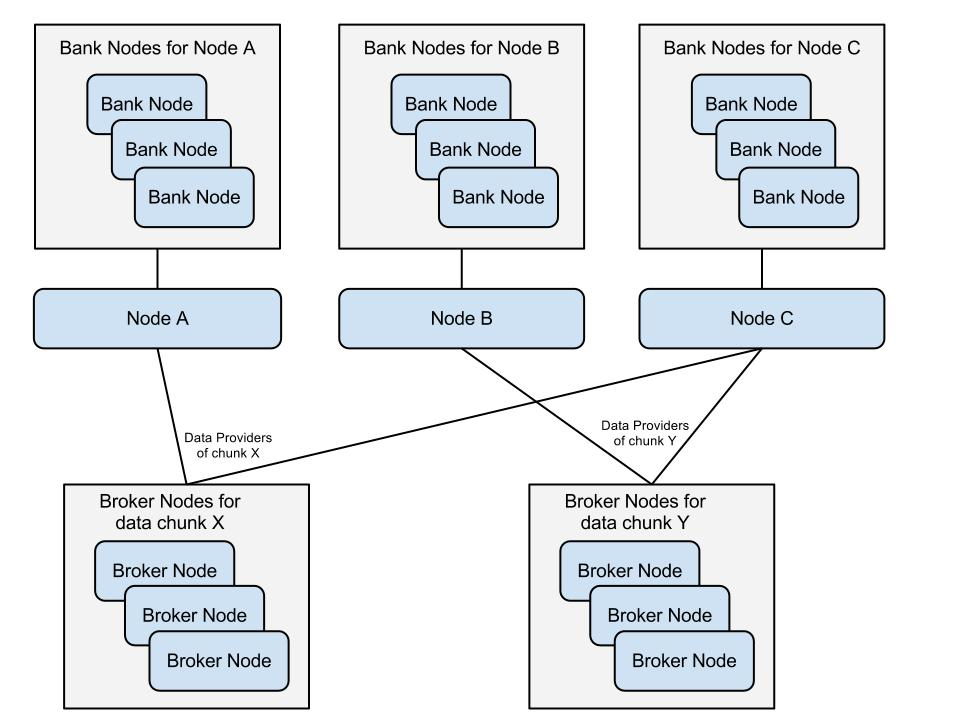
\includegraphics[height=65mm,width=65mm]{graphics/NodesSystemDiagram.jpg}
  \caption{Nodes system diagram depicting the relationships between the various node roles.  Each node has an associated set of bank nodes.  Each data chunk has an associated set of brokers.  Each data chunk also has a set of data providers that is maintained by the brokers for the data.
}
  \end{center}
\end{figure}


\subsection{Node Identity}
Each node in the system has a unique identity that consists of a node ID, bank set ID, and a pair of signing keys.  When a new node first joins the network it has no identity and no currency. In order to establish a identity a new node must first generate a public/private signing key pair.  The node and bank set IDs are derived from the public signing key using a cryptographic hash.  This prevents the node from choosing a specific node and bank set id.  If nodes were able to select these ids a malicious user could create and control a node along with its bank set.  After generating the key pair the new node can initialize a bank set by sending its public signing key to nodes with an ID near its bank set id.  These nodes will check to ensure that they should be a member of the bank set by searching for nodes with an id that is closer to the bank set id.  

When two nodes connect they exchange information that can be used to verify node identity.  This includes the node and bank set ids as well as the peer's node id signed using the other node's private signing key.  If the signature on the node id is valid then the other node's identity is verified.  A node can verify the signature of another node by requesting the public signature key from the nodes's bank nodes.

\subsection{Currency}
Currency in the system exists as discrete units.  A node never has direct access to the currency it owns.  The bank nodes of the node are responsible for performing the actual currency transfers.  Only currency transfers that are part of a brokered transaction are authorized. This makes bribry more difficult.  The which owns the currency along with a threshold of brokers for a data chunk must provide a signed transfer authorization before bankers will accept a transaction.  To ensure that a node cannot bribe it own bankers once a currency unit has been owned by a node it can never be transferred to one of its bankers.

\subsection{Currency Creation}
Currency that is permanently taken out of circulation must be replaced to ensure the system continues to function.  Currency can taken out of circulation when nodes leave the system or hoard currency as part of an attack on the system.  Bank nodes are responsible for minting new currency.  A threshold of bank nodes may periodically authorize the creation of currency for new nodes and nodes with a good reputation. As an additional precaution currency creation authorizations should also be signed by the bank nodes of the bank nodes to a desired depth.

\subsection{Secret Sharing}
In our system secret sharing is used to distribute the broker role to multiple nodes. Secret sharing is a method used in distributing a secret amongst a group of participants, each of whom is allocated a "share" of the secret.  The secret can be reconstructed only when a sufficient number of shares are combined together.  As a result, the individual shares, alone, provide no useful information.  

\subsection{Brokers}
Nodes that have an ID close to the ID of a data chunk must act as brokers for that data. Each broker maintains a list of nodes that are registered as providers for the data.  Each broker also stores a share of the encryption key that is used to encrypt the data as well as the hash of the encrypted data. The hash and decryption key share can be obtained from any data provider or broker for the data.  The decryption key share provided to the broker is based on the broker's ID.  This ensures that each broker can only obtain one share of the decryption key.

\subsection{Brokered Data Transfer}
In order to initiate a data transfer a consumer must first locate brokers for the data.  This can be done by searching for nodes with an ID close to the data id.  Once a sufficient number of brokers have been located the consumer can obtain a list of data providers and select a data provider for the transfer.  The consumer can then send a signed data request to the provider.  The request may be accepted or rejected based on a number of factors including:
\begin{itemize}
\item The amount of currency offered
\item The reputation of the data consumer
\item The reputation of the brokers selected by the data consumer
\item The current load on the data provider
\end{itemize}
If the provider accepts the request it will send the signed request that the consumer provided to the consumer's bank nodes to place a temporary reserve on the currency.  The provider will then send the encrypted data to the consumer.  After receiving the data the consumer will send a hash of the received data along with a signed currency transfer authorization to each broker. Each broker will verify the encrypted data hash and currency transfer authorization.  If they are valid the broker will send a signed share of the decryption key to the consumer and a signed copy of the currency transfer authorization to the data provider.  When the data consumer receives a sufficient number of decryption key shares it can recover the key and decrypt the data.  When the data provider receives a sufficient number of currency transfer authorizations it can submit them to the consumer's bank nodes.

\begin{figure}
  \begin{center}
    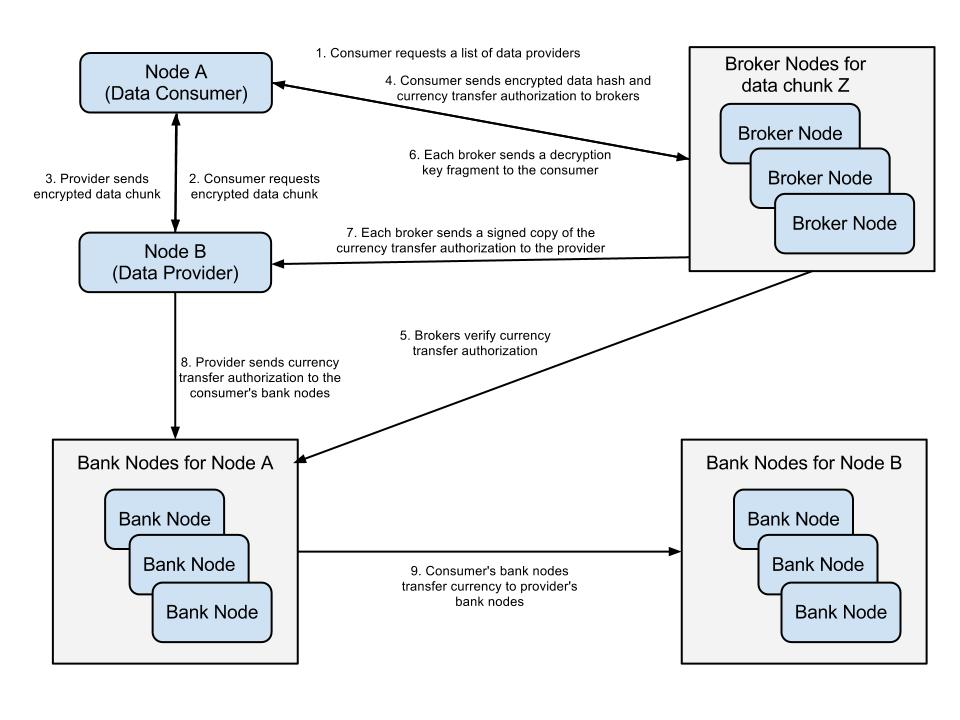
\includegraphics[height=85mm,width=65mm]{graphics/BrokeredDataTransfer.jpg}
  \caption{A brokered data transfer.}
  \end{center}
\end{figure}

\subsection{Storage}
We have designed an interface to a data storage object that takes a node id and reads or writes a data chunk.  In our system, the idea is that a node wishes to use their available storage space to store data chunks so that they may provide data to others in exchange for currency.  The user can then use the currency to get data they don't have. 

\subsection{Node Reputation}
When nodes initiate a transaction they exchange signed transaction records which contain:
\begin{itemize}
\item The date/time the transaction began
\item The ID, bank set ID, and role of each node involved
\item The transaction expiration date
\item Any other supporting information
\end{itemize}
When the transaction is complete each node appends a signed satisfaction statement to the record and submits the record to the appropriate bank nodes. If the satisfaction statement indicates a complaint it must also be signed by a threshold of the bank nodes of the complaining node.  This provides a mechanism for bank nodes to stop complaints for nodes that have a high ratio of complaints to completed transactions.  Signed transaction records can sometimes be used as evidence for a complaint.  For example if a node makes contradictory statements to different nodes or to the same node at different points in time the signed transaction records can be used to prove that fact.  Depending on the nature of the complaint nodes against which a complaint with evidence has been made may be removed from the system.  Each node acts as one of its bank nodes.  This allows the node to collect and provide the information needed to check it bank nodes.

\subsection{Node Role Motivations}
It is reasonable to expect that nodes would not take on the broker and bank node roles unless a motivation exists for them to do so.  In our system nodes must perform these roles in order to maintain a good reputation.  When a node fails to participate in a transaction the other nodes in its set will report the fact to the bank nodes of the node.  If the node is inactive its bank nodes will return this information and the other nodes in the set will not report inactivity for that node for a specified time interval.  If the node was active then a complaint will be registered against the node which will lower its reputation.  The bank nodes of a node have the information they need to determine if the node was active or inactive.  A node is considered active if it has recent incoming or outgoing currency transfers.

\subsection{Automated transaction valuation based on reputation parameters}
Because of the risk of fraud inherent in peer-to-peer systems data consumers should attempt to use the most reputable data providers available.  It is expected that highly reputable data providers should receive more currency units per transaction than less reputable data providers.  Conversely data providers may charge less to more reputable data consumers.  
Data consumers can use the following information when determining how much currency to offer a data provider for a transfer:
\begin{itemize}
\item The number and reputation of nodes which can provide the data
\item The number and reputation of brokers available for the data
\item The number of nodes which are currently consuming the data
\item A measure of the value the consumer places on obtaining the data
\end{itemize}
The state of the network is expected to be constantly changing.  Data consumers should be capable of automatically adjusting their valuations as network conditions change. 

\subsection{Determining Broker / Bank Set Size}
The size of the broker and bank sets are automatically adjusted periodically.  The size of these sets should be large enough to ensure that uncooperative nodes in the set will not be numerous enough to interfere with operations.  The sets should also not be larger than is necessary to minimize overhead.  The members of a set collectively decide whether new members should be added or existing members removed based on the recent reliability statistics of the members of the set.  One basic metric is the ratio of successful transactions to number of transactions.  If the overall reliability of the set is too low low reliability members can be replaced with new members.  If the overall reliability is high and the set is large low reliability members can be removed.  The initial size of a set is determined by querying the size of other sets.

\subsection{Attack Analysis}

In order for our system to be successful it must enforce cooperation even when most nodes act only in their own self interest.  Some nodes may act with the sole goal of disrupting the system.  

Bank Nodes:
Bank nodes could collude to provide inaccurate positive reputation information
Bank nodes could collude to provide inaccurate negative reputation information
Bank nodes could collude to transfer the same currency unit to different nodes
Bank nodes could collude to deny a node access to its currency

Brokers:
Brokers could collude to authorize transactions without valid currency
Brokers could collude to authorize transactions with an invalid encrypted data hash
Brokers could collude to sell their shares of the decryption key 
Brokers could collude to reject all transactions

Data Providers:
Data Providers could sell the data decryption key alone without providing data

%----------------------------------------------------------------------
% SECTION III: Simulation
%----------------------------------------------------------------------
\subsection{Simulation Framework}
In order to evaluate the effectiveness of our system design we will be implementing a simulated peer to peer cloud storage network.  This approach will allow us to quickly test many scenarios involving a large number of nodes and data transfers.  In order to implement the simulation we will be combining fully functional component implementations with simulation component implementations.  The simulation will be driven by simulated nodes with various behaviors.  These simulated nodes will perform the actions that they typically would in the real system and may be fully cooperative or uncooperative in various ways.  A simulated node is made by combining simulated behaviors for each of the roles the node may take in the system.

\begin{center}
  \begin{tabular}{ p{6.25cm} }
    \bf Data Consumer Node \\ \hline
    \hline
    Fully cooperative \\ \hline
    Fails to provide payment to the broker with a given probability \\ \hline
    Fails to provide correct payment amount to the broker with a given probability \\ \hline
    Fails to provide payment transfer for the correct node to the broker with a given probability \\ \hline
    Permanently stops consuming data with a given probability \\
    \hline
  \end{tabular}
\end{center}

\begin{center}
  \begin{tabular}{ p{6.25cm} }
    \bf Data Provider Node \\ \hline
    \hline
    Fully cooperative \\ \hline
    Fails to provide correct data with a given probability \\ \hline
    Provides data at a slow rate with a given probability \\ \hline
    Permanently stops providing data with a given probability \\ \hline
  \end{tabular}
\end{center}

\begin{center}
  \begin{tabular}{ p{6.25cm} }
    \bf Bank Node \\ \hline
    \hline
    Fully cooperative \\ \hline
    Fails to store currency transfer authorizations with a given probability \\ \hline
    Accepts invalid transfer authorizations with a given probability \\ \hline
    Declines valid transfer authorizations with a given probability \\ \hline
    Fails to forward transferred currency units to the proper bank nodes with a given probability \\ \hline
    Permanently stops providing bank node functions with a given probability \\ \hline
  \end{tabular}
\end{center}

\begin{center}
  \begin{tabular}{ p{6.25cm} }
    \bf Broker Node \\ \hline
    \hline
    Fully cooperative \\ \hline
    Sends decryption key to consumer without proper payment with a given probability \\ \hline
    Sends decryption key to consumer without forwarding payment transfer to bank nodes with a given probability \\ \hline
    Sends invalid decryption key to consumer after authorizing payment \\ \hline
    Fails to validate that payment transfer is for correct provider with a given probability \\ \hline
  \end{tabular}
\end{center}


During each simulation the following statistics will be collected to measure the effectiveness of the system:

\begin{itemize}
\item The number of invalid bytes received by cooperating consumers
\item The number of bytes received by cooperating consumers
\item The number of bytes sent by providers to consumers that did not pay
\item The number of bytes sent by providers
\item The number of bank node requests
\item The number of broker node requests
\item The number of data transfer requests
\end{itemize}

When a node joins the simulated network it will either be made a fully cooperative node or an uncooperative node.  The probability that a node will be uncooperative along with the behavior probabilities will be set based on the simulation parameters.

\subsection{Distributed Hash Table}
Kademlia was chosen as an alternative to Chord for use as the DHT serving node 
lookups.  It has several advantages over its more well-known brethren. 
~\cite{maymounkov} Lookups spread information about the network, reducing the 
traffic of overhead control information.  The use of the XOR metric to 
calculate distances between nodes provides for a more flexible and dynamic 
routing table, allowing it to send out multiple queries that are asynchronous.  
This completely sidesteps the problem of timeout delays, since the system can 
easily select the result of any of the asynchronous calls, or even send out new 
ones.  Furthermore, Kademlia's use of a single routing algorithm, as opposed to 
the dual gauge-and-pinpoint algorithms or other protocols, is both easier to 
understand and implement from a design perspective.


\subsection{Simulation Results}
Implementation of the simulation is currently in progress.

%----------------------------------------------------------------------
% SECTION IV: Conclusion
%----------------------------------------------------------------------
\section{Conclusion}
Milestone 3

\newpage

% try out a theorem...
%\newtheorem{theorem}{Theorem}

%\begin{theorem}[Theorem name]
%  Consider the system ...
%\end{theorem}

%\begin{proof}
%  The proof is trivial.
%\end{proof}

% do the bibliography:
\bibliographystyle{IEEEbib}
\bibliography{cs598}

% where ``my-bibliography-file.bib'' is the name of the file with all the 
% BibTeX entries.

% do the biographies...
%\begin{biography}{Gregory L. Plett}
%  A bio with no face...
%\end{biography}

% If you want a picture with your biography, then specify the name of
% the postscript file in square brackets. That is, uncomment the
% following three lines and change the name of "face.ps" to the name of 
% your file.
%\begin{biography}[face.ps]{Gregory L. Plett}
%  A bio with a face...
%\end{biography}

%----------------------------------------------------------------------
% FIGURES
%----------------------------------------------------------------------
% There are many ways to include figures in the text. We will assume
% that the figure is some sort of EPS file.
%
% The outdated packages epsfig and psfig allow you to insert figures
% like: \psfig{filename.eps} These should really be done now using the
% \includegraphics{filename.eps} command.  
%
% i.e.,
%
% \includegraphics{file.eps}
%
% whenever you want to include the EPS file 'file.eps'. There are many
% options for the includegraphics command, and are outlined in the
% on-line documentation for the "graphics bundle". Using the options,
% you can specify the height, total height (height+depth), width, scale,
% angle, origin, bounding box "bb",view port, and can trim from around
% the sides of the figure. You can also force LaTeX to clip the EPS file
% to the bounding box in the file. I find that I often use the scale,
% trim and clip commands.
% 
% \includegraphics[scale=0.6,trim=0 0 0 0,clip=]{file.eps}
% 
% which magnifies the graphics by 0.6 (If I create a graphics for an
% overhead projector transparency, I find that a magnification of 0.6
% makes it look much better in a paper), trims 0 points off
% of the left, bottom, right and top, and clips the graphics. If the
% trim numbers are negative, space is added around the figure. This can
% be useful to help center the graphics, if the EPS file bounding box is
% not quite right.
% 
% To center the graphics,
% 
% \begin{center}
% \includegraphics...
% \end{center}
% 
% I have not yet written good documentation for this, but another 
% package which helps in figure management is the package ieeefig.sty,
% available at: http://www-isl.stanford.edu/people/glp/ieee.shtml
% Specify:
% 
%\usepackage{ieeefig} 
% 
% in the preamble, and whenever you want a figure,
% 
%\figdef{filename}
% 
% where, filename.tex is a LaTeX file which defines what the figure is.
% It may be as simple as
% 
% \inserteps{filename.eps}
%
% or
% \inserteps[includegraphics options]{filename.eps}
% 
% or may be a very complicated LaTeX file. 

\end{document}
